در ابتدا تعداد بلوک‌ها را بدست می‌آوریم:

\setLTR
$
\frac{256Byte}{32Bit} = \frac{256 \times 8}{32} = 64
$
\setRTL

چون حافظه نهان ما از نوع انجمنی دو انتخابی است پس هر مجموعه 2 بلوک دارد. پس در کل 32 مجموعه خواهیم داشت که برای index آن نیازمند 5 بیت هستیم. همچنین چون بلوک‌های 4 بایتی داریم، به 2 بیت برای offset نیازمند هستیم. پس تعداد بیت‌های Tag برابر است با:

\setLTR
$
32 - 2 - 5 = 25Bit
$
\setRTL

حال آدرس‌های داده شده بررسی می‌کنیم:

\setLTR
\qquad\qquad\qquad\qquad\qquad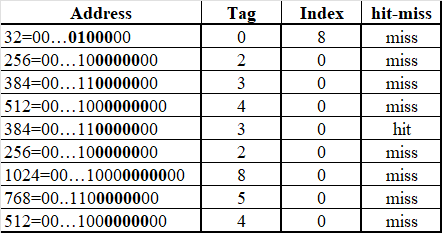
\includegraphics[width=0.5\linewidth]{figs/1.png}
\setRTL

در آخر حافظه ما به این صورت خواهد بود:

\begin{itemize}
	\item
	 مجموعه 0 : ---و32
	 \item 
	 مجموعه 8 : 512 و 768
	 \item 
	 مجموعه 1 تا 7 : --- و ---
\end{itemize}